\section{Results}
\label{sec:results}

\subsection{Clean baseline, and what it already tells us}

Table~\ref{tab:baseline} is the clean zero-shot baseline, before any attack. Two
rows matter more than the accuracy column.

\textbf{Phi-3.5-mini is a cautious detector on e-mail.} Its precision is high
(0.896) but it misses 80 of the 200 phishing messages, a catch rate of 60.0\%.
It is the model that leaves the most malicious mail in the analyst's queue before
any attack happens.

\textbf{SmolLM2-1.7B is a degenerate detector.} It reaches a catch rate of 98.5\%
on phishing e-mail, but its precision is 0.510 and its confusion matrix shows 189
false positives against 11 true negatives on the benign class: it calls nearly
every message malicious. A detector that says \emph{malicious} almost always is
hard to flip towards \emph{benign}, and every robustness number for it has to be
read against that fact.

Qwen2.5-3B is the strongest and most balanced classifier of the three (F1 0.923
on e-mail, 0.857 on SMS).

\begin{table*}[t]
\centering
\small
\caption{Clean zero-shot baseline on the frozen 800-row evaluation split (400 rows per task, 200 malicious). ``Catch'' is recall on the malicious class and is the denominator every ASR in this paper is conditional on.}
\label{tab:baseline}
\begin{tabular}{llcccccc}
\toprule
\textbf{Task} & \textbf{Model} & \textbf{Acc.} & \textbf{Prec.} & \textbf{Rec.} & \textbf{F1} & \textbf{TP/FP} & \textbf{Catch} \\
\midrule
 SMS smishing & Phi-3.5-mini-instruct & 0.772 & 0.751 & 0.815 & 0.782 & 163/54 & 81.5\% \\
  & Qwen2.5-3B-Instruct & 0.843 & 0.787 & 0.940 & 0.857 & 188/51 & 94.0\% \\
  & SmolLM2-1.7B-Instruct & 0.525 & 0.514 & 0.925 & 0.661 & 185/175 & 92.5\% \\
\midrule
 Phishing email & Phi-3.5-mini-instruct & 0.765 & 0.895 & 0.600 & 0.719 & 120/14 & 60.0\% \\
  & Qwen2.5-3B-Instruct & 0.920 & 0.892 & 0.955 & 0.923 & 191/23 & 95.5\% \\
  & SmolLM2-1.7B-Instruct & 0.520 & 0.510 & 0.985 & 0.672 & 197/189 & 98.5\% \\
\bottomrule
\end{tabular}
\end{table*}


\subsection{Character-level evasion}

Table~\ref{tab:asr-char} reports the character-level attack. Of 1{,}044 caught
messages attacked, 12 flipped: an aggregate of 1.1\%. Per row the ASR lies
between 0.0\% and 5.0\%, and under a 15\% budget the mean edit actually spent was
13.3--13.6\% of characters, with no row above the budget (maximum 13.6\%).

The highest row is Phi-3.5-mini on phishing e-mail: 6 flips in 120 attacked
messages, 5.0\% (95\% CI 2.3--10.5). This is the model with the lowest catch rate
on that task. The model that catches 95.5\% of e-mail (Qwen2.5-3B) flips once in
191 attacks, and on SMS it flips zero times in 188 attempts. A zero is reported
as a bounded measurement, not as a proof: the Wilson upper bound for that row is
2.0\%.

\begin{table*}[t]
\centering
\small
\caption{Character-level evasion under a 15\% edit budget. ASR is flips / samples attacked, where only samples the clean model classified malicious are attacked and each original is re-queried. CI is a 95\% Wilson interval.}
\label{tab:asr-char}
\begin{tabular}{llccccccc}
\toprule
\textbf{Task} & \textbf{Model} & \textbf{Attacked} & \textbf{Flips} & \textbf{ASR} & \textbf{95\% CI} & \textbf{Pert.} & \textbf{Jacc.} & \textbf{Catch} \\
\midrule
 SMS smishing & Phi-3.5-mini-instruct & 163 & 3 & 1.8\% & 0.6--5.3 & 13.3\% & 0.328 & 81.5\% \\
  & Qwen2.5-3B-Instruct & 188 & 0 & 0.0\% & 0.0--2.0 & 13.5\% & 0.322 & 94.0\% \\
  & SmolLM2-1.7B-Instruct & 185 & 1 & 0.5\% & 0.1--3.0 & 13.5\% & 0.317 & 92.5\% \\
\midrule
 Phishing email & Phi-3.5-mini-instruct & 120 & 6 & 5.0\% & 2.3--10.5 & 13.5\% & 0.322 & 60.0\% \\
  & Qwen2.5-3B-Instruct & 191 & 1 & 0.5\% & 0.1--2.9 & 13.6\% & 0.303 & 95.5\% \\
  & SmolLM2-1.7B-Instruct & 197 & 1 & 0.5\% & 0.1--2.8 & 13.4\% & 0.311 & 98.5\% \\
\bottomrule
\end{tabular}
\end{table*}


\subsection{Word-level evasion}

Table~\ref{tab:asr-word} applies the same budget to whole words. Of 1{,}035
caught messages, 28 flipped --- more than twice the character-level count ---
while changing only 6.2--9.2\% of words, roughly half the unit budget the
character attack spent. Word-set Jaccard stays at 0.916--0.950, so the messages
are 92--95\% word-identical to what the model had already caught.

The ranking changes. The character attack leaves Qwen2.5-3B on SMS at zero flips;
the word attack flips 6 of 186 (3.2\%, CI 1.5--6.9). A replaced word carries
meaning that a single letter does not: swapping a suspicious verb for a neutral
synonym, or deleting the word that carried the urgency, moves a verdict that typo
noise leaves alone.

\begin{table*}[t]
\centering
\small
\caption{Word-level evasion under the same 15\% budget (synonym swap, deletion, duplication, swap). Jaccard is word-set overlap; no semantic-similarity model is used anywhere in this study.}
\label{tab:asr-word}
\begin{tabular}{llccccccc}
\toprule
\textbf{Task} & \textbf{Model} & \textbf{Attacked} & \textbf{Flips} & \textbf{ASR} & \textbf{95\% CI} & \textbf{Pert.} & \textbf{Jacc.} & \textbf{Catch} \\
\midrule
 SMS smishing & Phi-3.5-mini-instruct & 161 & 6 & 3.7\% & 1.7--7.9 & 9.0\% & 0.918 & 81.5\% \\
  & Qwen2.5-3B-Instruct & 186 & 6 & 3.2\% & 1.5--6.9 & 9.2\% & 0.916 & 94.0\% \\
  & SmolLM2-1.7B-Instruct & 184 & 3 & 1.6\% & 0.6--4.7 & 8.8\% & 0.916 & 92.5\% \\
\midrule
 Phishing email & Phi-3.5-mini-instruct & 118 & 6 & 5.1\% & 2.4--10.7 & 6.3\% & 0.945 & 60.0\% \\
  & Qwen2.5-3B-Instruct & 190 & 5 & 2.6\% & 1.1--6.0 & 6.2\% & 0.950 & 95.5\% \\
  & SmolLM2-1.7B-Instruct & 196 & 2 & 1.0\% & 0.3--3.6 & 6.3\% & 0.948 & 98.5\% \\
\bottomrule
\end{tabular}
\end{table*}


\subsection{Budget accounting}

Table~\ref{tab:budget} is the accounting check, and Figure~\ref{fig:budget} draws
the same accounting instead of summing it: one point per model, task and attack,
with the budget spent on the horizontal axis. Both modes stay inside the shared
budget, and the word attack reaches a similar number of flips with about half the
share of units changed. That imbalance is the paper's main measured point: for
these models, \emph{what} is changed matters more than \emph{how much}.

\begin{table}[t]
\centering
\small
\caption{Edit budget actually spent, by attack mode. The budget is one shared 15\% allowance per sample; the measured rate is the exact Levenshtein distance divided by the original length (characters or words).}
\label{tab:budget}
\begin{tabular}{lcccc}
\toprule
\textbf{Mode} & \textbf{Samples} & \textbf{Flips} & \textbf{Mean pert.} & \textbf{Max pert.} \\
\midrule
 Character & 1044 & 12 & 13.5\% & 13.6\% \\
 Word & 1035 & 28 & 7.6\% & 9.2\% \\
 Saliency & 1001 & 46 & 9.3\% & 12.9\% \\
\midrule
\multicolumn{2}{l}{Total} & 86 & & \\
\bottomrule
\end{tabular}
\end{table}


\IfFileExists{figures/fig_budget.pdf}{%
\begin{figure}[t]
\centering
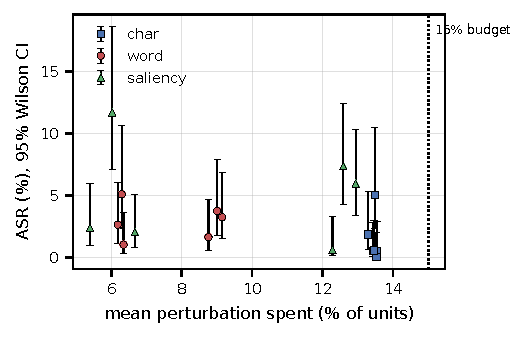
\includegraphics[width=\columnwidth]{figures/fig_budget}
\caption{Each point is one (model, task, attack) cell: the edit actually spent on
the horizontal axis, the ASR with its 95\% Wilson interval on the vertical one.
The dotted line is the 15\% budget. Points to the left of a vertical pair are the
same amount of visible change bought at half the unit cost \--- the word attack's
advantage is horizontal as well as vertical.
\label{fig:budget}}
\end{figure}}{}

\IfFileExists{figures/fig_asr.pdf}{%
\begin{figure*}[t]
\centering
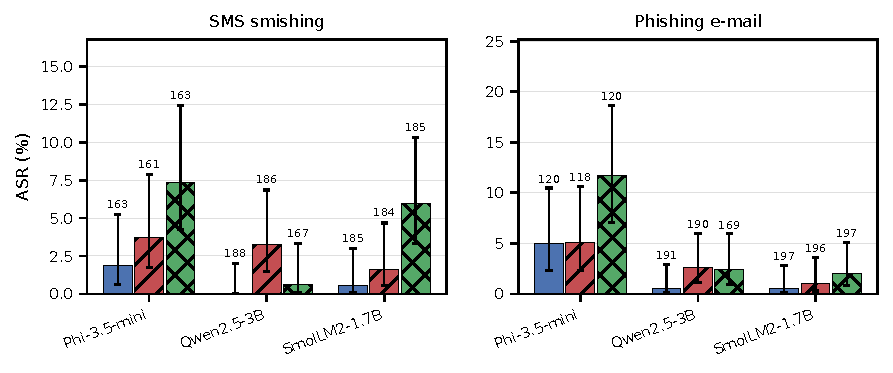
\includegraphics[width=\textwidth]{figures/fig_asr}
\caption{Attack success rate per model, task and attack mode, with 95\% Wilson
intervals on the flip count. Solid blue bars are the character attack, hatched
red bars the word attack, and green cross-hatched bars the saliency-guided word
attack of \S\ref{sec:saliency}, which is drawn here for comparison but costs
22.9 model queries per message against 3.9 for the two random attacks, so the
bars are not a comparison at equal cost. The number above
each interval is the total count:
the messages that model had caught on the clean text and that were therefore
attacked. A cell at zero is drawn with its interval, not as a point at the
origin, because 0/188 is a bounded measurement rather than a proof of
robustness.\label{fig:asr}}
\end{figure*}}{}

\subsection{What predicts fragility}
\label{sec:fragility}

Across the six model--task cells, the ASR follows how close a model sits to its
decision boundary rather than how accurate it is. Phi-3.5-mini has the highest
character ASR on e-mail (5.0\%) and the weakest recall there (0.600). SmolLM2-1.7B
has the highest recall (0.985) and among the lowest ASR (0.5\% on e-mail) ---
because its decision rule is nearly constant. A small edit either does nothing
or, as in the case of the 2 of 196 word attacks that flipped it, pushes a
barely-considered verdict across the line. Neither behaviour is robustness in the
sense a deployment cares about.

\subsection{Interval discipline}

Figure~\ref{fig:asr} collects all twelve random-attack cells and the three
saliency cells in one panel, with the interval drawn on every bar, so the
comparison below can be read at a glance rather than row by row.

Because the flip counts are small, we do not rank models on point estimates. Of
the twelve pairs of rows sharing a task and one of the two random attack modes,
9 of 12 have intervals that overlap by more than half the narrower interval, so
within-task ordering is suggestive rather than established. The exceptions are
informative: under the character attack on phishing e-mail, Phi-3.5-mini's
interval overlaps Qwen2.5-3B's by 21.3\% and SmolLM2-1.7B's by 18.7\% of the
narrower width --- the one separation that survives the uncertainty is exactly
the boundary-proximity effect of \S\ref{sec:fragility}.

What the intervals do establish is magnitude, and the magnitude depends on the
search. No random-edit cell exceeds 10.7\% at its upper bound; the saliency-guided
cells of \S\ref{sec:saliency} reach 18.6\%. The claim ``under a 15\% edit budget
a random edit leaves these models close to robust'' survives the uncertainty; the
claim ``model A is more robust than model B'' does not, for most pairs, and
neither claim extends to a better search.

\subsection{Is the difference between the two modes real?}
\label{sec:pairs}

Comparing a 3.7\% cell with a 1.8\% cell as if they were independent samples is
the wrong test: both attacks ran on the \emph{same} messages, so the flips are
paired, and the pairing is what makes a small difference measurable. We pair the
per-sample outcomes on the message identifier and report the counts of messages
the two attacks disagree on, an exact McNemar test, and a paired bootstrap of the
difference in risk over messages.

% Generated by src/make_paper_tex.py from results/paired_tests.csv.
Pairing the two attacks on the messages both of them attacked, the word attack flips 26 messages the character attack leaves alone, and the character attack flips 10 that the word attack leaves alone (exact McNemar $p = 0.011$ over the pooled discordant counts).
Per cell, 1 of 6 show a significant paired difference at $p<0.05$: SMS smishing/Qwen2.5-3B-Instruct. The rest are underpowered rather than contradictory, and the pooled test is a description of the direction because the cells reuse the same messages across models.


\begin{table*}[t]
\centering
\small
\caption{Paired comparison of two attack modes on the same messages. Only the discordant counts carry information about the difference: A-only flips happened under the first mode and not the second, B-only the reverse. The p-value is an exact McNemar test (binomial on the discordant counts); the interval is a percentile bootstrap over messages of the paired risk difference.}
\label{tab:pairs}
\begin{tabular}{lllccccccc}
\toprule
\textbf{A vs B} & \textbf{Task} & \textbf{Model} & \textbf{Paired} & \textbf{A flips} & \textbf{B flips} & \textbf{Risk diff.} & \textbf{95\% CI} & \textbf{A/B only} & \textbf{$p$} \\
\midrule
 saliency vs word & Phishing email & Phi-3.5-mini-instruct & 118 & 14 & 6 & +6.8 & +1.7 to +11.9 & 9/1 & 0.021 \\
 saliency vs word & Phishing email & Qwen2.5-3B-Instruct & 169 & 4 & 1 & +1.8 & -0.6 to +4.7 & 4/1 & 0.375 \\
 saliency vs word & Phishing email & SmolLM2-1.7B-Instruct & 196 & 3 & 2 & +0.5 & -1.0 to +2.0 & 2/1 & 1.000 \\
 saliency vs word & SMS smishing & Phi-3.5-mini-instruct & 161 & 12 & 6 & +3.7 & +0.6 to +7.4 & 7/1 & 0.070 \\
 saliency vs word & SMS smishing & Qwen2.5-3B-Instruct & 167 & 1 & 1 & +0.0 & -1.8 to +1.8 & 1/1 & 1.000 \\
 saliency vs word & SMS smishing & SmolLM2-1.7B-Instruct & 184 & 11 & 3 & +4.3 & +1.1 to +8.2 & 10/2 & 0.039 \\
 word vs char & Phishing email & Phi-3.5-mini-instruct & 118 & 6 & 6 & +0.0 & -5.1 to +5.1 & 5/5 & 1.000 \\
 word vs char & Phishing email & Qwen2.5-3B-Instruct & 190 & 5 & 1 & +2.1 & +0.0 to +4.7 & 5/1 & 0.219 \\
 word vs char & Phishing email & SmolLM2-1.7B-Instruct & 196 & 2 & 1 & +0.5 & -1.0 to +2.5 & 2/1 & 1.000 \\
 word vs char & SMS smishing & Phi-3.5-mini-instruct & 161 & 6 & 3 & +1.9 & -1.2 to +5.0 & 5/2 & 0.453 \\
 word vs char & SMS smishing & Qwen2.5-3B-Instruct & 186 & 6 & 0 & +3.2 & +1.1 to +5.9 & 6/0 & 0.031 \\
 word vs char & SMS smishing & SmolLM2-1.7B-Instruct & 184 & 3 & 1 & +1.1 & -1.1 to +3.3 & 3/1 & 0.625 \\
\bottomrule
\end{tabular}
\end{table*}


The honest reading is narrower than the raw table suggests. The direction is
consistent --- word-level edits flip more messages than character-level ones in
five of six cells and never fewer --- but only one cell is significant on its
own, because there the character attack flipped nothing at all. What survives is
a pooled statement about this corpus and these three models, not a per-model
ranking, and the interval widths in Table~\ref{tab:pairs} say the same thing.
